\subsection{Subsystem $<$Controller$>$}

\subsubsection{Detailed Design Diagram}
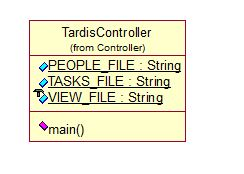
\includegraphics{subsystems/diagrams/controller_class_diagram.jpg}

UML class diagram depicting the internal structure of the subsystem,
accompanied by a paragraph of text describing the rationale of this design.

The controller is resposible for loading the data and giving it to the view.

\subsubsection{Units Description}

\emph{TardisController}\\
Functions:\\
\begin{tabular}{| l | l | l | l |}
\hline
Name & Parameters & Pre-conditions & Post-conditions\\
\hline
\multirow{2}{*}{main} & String[] args & Requires Nothing & Ensures that the data has been loaded\\ 
			 &  & & and passed to the main view
\\
\hline
\end{tabular}\\
\\
Attributes:\\
\begin{tabular}{| l | l |}
\hline
Name & Description\\
\hline
String PEOPLE\_FILE & The assumed name of the file containing the people.\\
\hline
String TASKS\_FILE & The assumed name of the file containing the tasks.\\
\hline
String VIEW\_FILE & The assumed name of the file in which to dump the people.\\
\hline 
\end{tabular}

Purpose: The main program. Loads the people and tasks from the files and passes them to the main view.

List each class in this subsystem and write a short description of its purpose,
as well as notes or reminders useful for the programmers who will implement them.
List all attributes and functions of the class.